\chapter{Probability}




\section{Information Theory}

When we communicate a message, we want as much useful information as possible to get through. In Shannon's theory to transmit one bit of information means to reduce the receiver uncertainty by a factor of 2. For example, if the weather has a random 50/50 chance of being either sunny or rainy every day and a weather stations tells you that it's going to rain tomorrow they have reduced your uncertainty by a factor of 2. The weather station then has send you a single bit of useful information.

\noindent We can find the number of bits of information that were actually communicated by computing:

$$I(x) = log_{2} \left( \frac{1}{P(x)} \right)  = -log_{2} \left( P(x) \right)$$

where $P(x)$ is the probability of the event $x$.


\noindent The basic intuition behind information theory is that learning an unlikely event is more informative that learning about a likely event.

\subsection{Entropy}

Self information deals only with a single outcome. We can quantify the amount of uncertainty or randomness in an entire probability distribution using the Shannon Entropy.

$$ H(P) = -\mathbb{E}_{x \sim p} \left[log_2 P(x) \right] = -\int_x {P(x)log_2\left(P(x)\right)dx} $$

\noindent The Shannon entropy of a distribution is the expected amount of (self-)information in an event $x$ drawn from distribution $P(x)$. Basically, it quantifies how much information is needed to describe or predict the outcome  of events governed by that distribution. Distributions that are nearly deterministic have low entropy. Distributions that are closer to uniform have high entropy. Therefore the higher the entropy, the higher is the uncertainty. Notice that if $P(x)$ is a discrete distribution the expected value will be the mean of $-P(x)log_2(P(x))$. 

\begin{figure}[h]
    \centering
    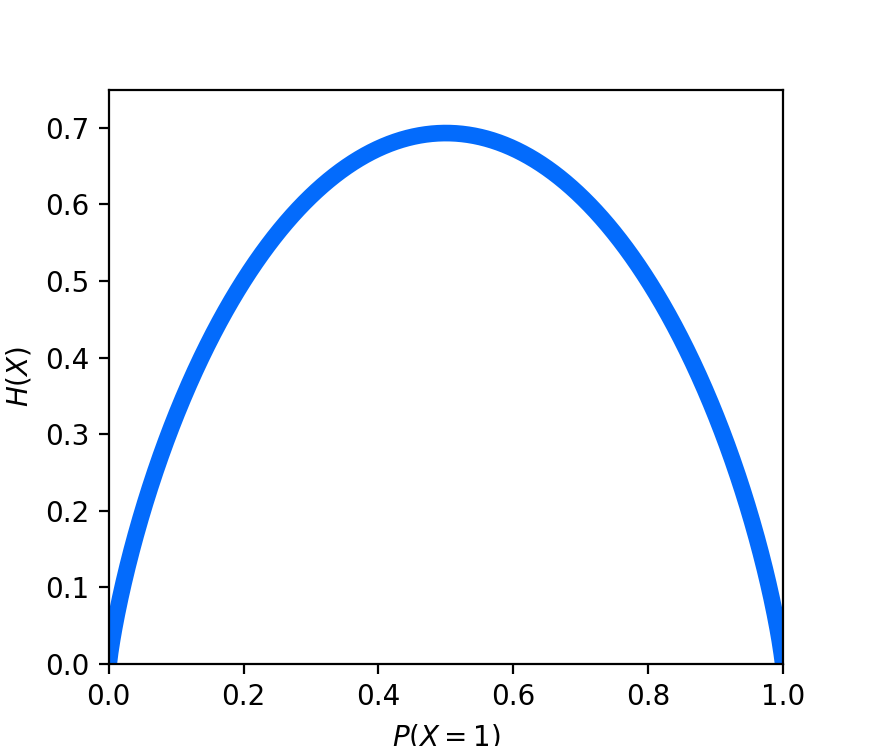
\includegraphics[width=4.5cm]{Plots/self-entropy.png}
    \caption{Shannon Entropy of a coin flip graphed versus the bias of the coin $P(x=1)$, where $x=1$ represents a result of heads.}
\end{figure}

\newpage
\subsection{Kullback-Leibler Divergence \& Cross-Entropy}

We can express cross entropy as the average number of bits needed to encode events from the true distribution $P(x)$ using the predicted distribution $Q(x)$. Cross-entropy is typically used as a loss function in supervised learning, aiming to minimize the difference between the predicted and true distributions. Cross-Entropy can also be seen as a way to measure the dissimilarity between two probability distributions for a given random variable or set of events.

$$H(P, Q) = - \mathbb{E}_{x \sim p} [{log Q(x)}] = -\int_x {P(x)log_2\left(Q(x)\right)dx} $$

\noindent If our predictions are perfect the predicted distribution is equal to the true distribution, then the cross-entropy is simply equal to the entropy. But if they differ then the cross-entropy will be greater than the entropy. 

$$ H(P, Q) \geq H(P) $$

\noindent The amount of bits which the Cross-Entropy exceeds the Entropy is called the relative entropy or the Kullback-Leibler Divergence. It quantifies how much extra information (in bits) is needed to encode events from one distribution when we use a code optimized for another distribution.

$$ D_{KL} (P \vert \vert Q) = H(P, Q) - H(P) = \mathbb{E}_{x \sim p} \left[ \frac{\log(P(x)}{\log(Q(x))} \right] = \mathbb{E}_{x \sim p} \left[ \log(P(x)) - \log(Q(x))  \right] $$

\noindent Because the KL divergence is non-negative and measures the difference between two distributions, it is often conceptualized as measuring some sort of distance between these distributions. However, it is not a true distance measure because is not symmetric.

$$ D_{KL} (P \vert \vert Q) \neq D_{KL} (Q \vert \vert P)$$

\noindent The KL divergence is 0 if P and Q are the same distribution (discrete variables) or equal almost everywhere (continuous variables).

\noindent Minimizing the Cross-Entropy with respect to Q is equivalent to minimizing the KL divergence between P and Q (if P is given, $H(P)$ and $ \mathbb{E}_{x \sim p} \left[ \log(P(x))  \right] $ are constants). In other words, given two distributions if one is fixed (your data-set) then you can only consider the approximation (your model).

\section{Maximum Likelihood Estimator}

In Deep Learning we work with parametric models that depend on a certain number of parameters (weights). The learning will consist then in trying to learn the correct weights. This can be seen as trying to find the parameters that maximize the likelihood that the training data is explained by the model probability distribution $p_{model}(x)$. Basically, among all the possible models we can choose, we will choose the one that explains the training data better. The maximum likelihood estimator for $\theta$ is defined as:

$$\theta_{ML} = argmax_{\theta} ~ p_{model} (x, \theta) $$

If the training data is a set of observations drawn i.i.d from an unknown data generative distribution $p_{data} (x)$ this can be written as:

$$\theta_{ML} = argmax_{\theta} \prod_{i=1}^{m} p_{model} (x^{(i)}, \theta) $$

\noindent Maximum Likelihood Estimator is a special case of Maximum a Posteriori Estimation when this one has a uniform prior. Basically, this consist in estimating the single set of parameters $\theta$ that maximize the likelihood that the model distribution $p_{model}(x)$ is able to explain the distribution of the training data. Conversely, using the Bayesian approach we will return a probability distribution over $\theta$ that characterize the likelihood of each set of possible parameters being able to explain the distribution of the training data. 

\noindent The Bayesian approach gives us a better estimate that Maximum Likelihood Estimator but is computationally extremely demanding. In the case of Neural Networks it is unfeasible to compute it (we have an infinite amount of hypothesis). Nevertheless, Maximum Likelihood Estimator is already a very good estimator. Having the assumption that the model of the true probability distribution is included in the hypothesis space, the Maximum Likelihood Estimator will converge to the optimal model.


\noindent Taking the product over many probabilities is numerically unstable. To solve that we can work with
the logarithm instead since it is a monotonically increasing function.

$$ \theta_{ML} = \log \left( argmax_{\theta} \prod_{i=1}^{m} p_{model} (x^{(i)}, \theta) \right) =  argmax_{\theta} \sum_{i=1}^{m} \log \left( p_{model} (x^{(i)}, \theta) \right)    $$

\noindent We can divide by m to express Maximum Likelihood Estimator as an expectation over the training data:

$$ \theta_{ML} = argmax_{\theta} ~ \mathbb{E} \left[ \log \left( p_{model} (x^{(i)}, \theta) \right) \right]    $$


\noindent Notice that this is result is equivalent to maximize the negative Kullback-Leibler divergence. We can see that
since the Kullback-Leibler divergence is given by:

$$ D_{KL} (p_{data} \vert \vert p_{model}) = \mathbb{E}_{x \sim p_{data}} \left[ \log(p_{data}(x)) - \log(p_{model}(x))  \right] $$

\noindent The term on the left is a function only of the data generating process therefore when we train the
model we only need to minimize.

$$- \mathbb{E}_{x \sim p_{data}} \left[ log \left( p_{model} (x) \right) \right] $$

\noindent Therefore can see the Maximum Likelihood Estimator as minimizing the Kullback-Leibler, which we know that is equivalent to minimizing the dissimilarity between the empirical data distribution $p_{data}(x)$ and the model distribution $p_{model}(x)$. Ideally, we would like to match the true data generating distribution $p_{data}$, but we have no direct access to this distribution.

\subsection{Condition Probability}

The probability of some event given that some other event has happened is called the conditional
probability and can be calculated as:

$$ P(Y=y \vert X=x) = \frac  {P(Y=y, X=x)} {P(X=x)} $$

\noindent Any joint probability distribution over many random variables may be decomposed into conditional
distributions over only one variable:

$$ P(x^{(1)}, ..., x^{(n)}) = P(x^{(1)}) \prod_{i=1}^{m} P(x^{(i)} \vert x^{(1)}, ..., x^{(i-1)})   $$

This is known as the chain rule or product rule of probability.

\subsection{Conditional Log-Likelihood}

The MLE can be generalized to the case where our goal is to estimate a conditional probability $ P (y \vert x, \theta)$
in order to predict $y$ given $x$.

$$\theta_{ML} = argmax_{\theta} ~ P (y \vert x, \theta) $$

\noindent If the input examples are i.i.d

$$\theta_{ML} = argmax_{\theta} ~ \sum_{i=1}^{m} P (y^{(i)} \vert x^{(i)}, \theta) $$

\subsection{Example: Linear regression as maximum likelihood}

Linear regression may be justified as a maximum likelihood procedure. Instead of producing a single prediction $\hat{y}$, we now think of the model as producing a conditional distribution $p(y \vert x)$. For linear regression we have the assumption to have Gaussian noise on the target with same variance, therefore the output will be the mean of a Gaussian distribution where the variance is fixed to some constant:

$$ p(y \vert x) = N(y, \hat{y}(x, \theta), \sigma^2)  $$

\noindent Considering the examples are assumed to be i.i.d.

$$\theta_{ML} = argmax_{\theta} ~ \sum_{i=1}^{m} P (y^{(i)} \vert x^{(i)}, \theta) = argmax_{\theta} ~ \sum_{i=1}^{m} N(y^{(i)}; \hat{y} (x^{(i)}, \theta), \sigma^2) = $$ 

$$ \theta_{ML} = argmax_{\theta} ~ \sum_{i=1}^{m} log \left( \sqrt{\frac{1}{2 \pi \sigma^2}}  \exp{\left[ -\frac{1}{2 \sigma^2} (y^{(i)} - \hat{y}^{(i)})^2  \right]}  \right) $$

$$ \theta_{ML} = argmax_{\theta} ~ \sum_{i=1}^{m} \left[ log \left( \sqrt{\frac{1}{2 \pi \sigma^2}} \right) + log \left(  \exp{\left[ -\frac{1}{2 \sigma^2} (y^{(i)} - \hat{y}^{(i)})^2  \right]}  \right)  \right] $$

$$ \theta_{ML} = argmax_{\theta} ~ \sum_{i=1}^{m} \left[ log (1) - log \left( \sqrt{2 \pi \sigma^2} \right) + \left( -\frac{1}{2 \sigma^2} (y^{(i)} - \hat{y}^{(i)})^2  \right)  \right] $$

$$ \theta_{ML} = argmax_{\theta} ~ \sum_{i=1}^{m} \left[ - \frac{1}{2} log  \left( 2 \pi \sigma^2 \right) + \left( -\frac{1}{2 \sigma^2} (y^{(i)} - \hat{y}^{(i)})^2  \right)  \right] $$

$$ \theta_{ML} = argmax_{\theta} ~   - \frac{n}{2} log  \left( 2 \pi \sigma^2 \right) +  \sum_{i=1}^{m} \left( -\frac{1}{2 \sigma^2} (y^{(i)} - \hat{y}^{(i)})^2  \right)   $$

$$ \theta_{ML} = argmax_{\theta} ~   - \frac{n}{2} log  \left( 2 \pi \sigma^2 \right) - \frac{1}{2 \sigma^2}  \sum_{i=1}^{m} \left(  y^{(i)} - \hat{y}^{(i)}  \right)^2   $$

\noindent Now we take out the part of the equation that does not depend on $\theta$.

$$ \theta_{ML} = argmax_{\theta} ~   - \sum_{i=1}^{m} \left(  y^{(i)} - \hat{y}^{(i)}  \right)^2   $$

\newpage
\noindent Which is equivalent to the Mean Squared Error formula used in regression which is:

$$ \theta_{MSE} = argmin_{\theta} ~ \frac{1}{n} \sum_{i=1}^{n} (y^{(i)} - \hat{y}^{(i)}(x, \theta) )^2 $$

\noindent To sum up we can say that maximizing the log-likelihood with respect to $\theta$ yields the same estimate of parameters $\theta$ as does minimizing the Mean Squared Error. That is why we use the Mean Squared Error as our loss function for regression problems.





